\documentclass{../acm_proc_article-me11_tweaked}
\usepackage[usenames,dvipsnames,svgnames,table]{xcolor}
\usepackage{graphicx}
\usepackage{alltt}
\usepackage{url}
\usepackage{caption}
\DeclareCaptionType{copyrightbox}
\usepackage{subcaption}

\captionsetup{belowskip=4.5pt,aboveskip=2pt}

\def \rothead [#1]{\rotatebox[origin=l]{45}{#1}}
\renewcommand{\arraystretch}{1.5}

\begin{document}

\conferenceinfo{\textit{MediaEval 2013 Workshop,}}{October 18-19, 2013, Barcelona, Spain}

\title{Experiments in Diversifying Flickr Result Sets}

%
\def\sharedaffiliation{%
\end{tabular}
\begin{tabular}{c}}
%

\numberofauthors{7}
\author{
\alignauthor
Neha Jain\\
    \email{nj1g12@ecs.soton.ac.uk}
\and
\alignauthor
Jonathon S. Hare\\
    \email{jsh2@ecs.soton.ac.uk}
\and
\alignauthor
Sina Samangooei\\
    \email{ss@ecs.soton.ac.uk}
\and
\alignauthor
John Preston\\
    \email{jlp1g11@ecs.soton.ac.uk}
\and
\alignauthor
Jamie Davies\\
    \email{jagd1g11@ecs.soton.ac.uk}
\and
\alignauthor
David P. Dupplaw
    \email{dpd@ecs.soton.ac.uk}
\sharedaffiliation
    \affaddr{Electronics and Computer Science, University of Southampton, United Kingdom}
}

\additionalauthors{Additional author: Paul H. Lewis ({\texttt{phl@ecs.soton.ac.uk}})}

\maketitle
\begin{abstract}
The 2013 MediaEval Diversification task looked to tackling the problem of search result diversification of Flickr results sets formed from queries about geographic places and landmarks. In this paper we describe our approach of using a min-max similarity diversifier coupled with pre-filters and a reranker. We also demonstrate a number of novel features for measuring similarity to use in the diversification step.
\end{abstract}

%\keywords{Geotagging, Probability Density, Image Annotation}

\section{Introduction and Motivation}
The diversification of search results is increasingly becoming an important topic in the area of information retrieval. The 2013 MediaEval Diversification task~\cite{DIV2013} aimed to foster new multimodal approaches to the diversification of result sets from social photo retrieval. 

Our motivation for this task was to build on the diversification techniques we developed in ImageCLEF'09~\cite{ecs17993} by incorporating truly multimodal data. We were also motivated to explore how the precision of the search results could be improved by filtering and re-ranking prior to the diversification step, thus minimising the loss in precision usually seen when diversification is applied.

\section{Methodology}\label{sec:meth}
In terms of overall approach, after a number of experiments, we settled on the workflow illustrated in Figure~\ref{fig:overview}. In order to improve precision, we applied filters to the input results list to remove images unlikely to be relevant, and for the runs that allowed use of the text and metadata, we reranked the results before applying diversification. To diversify the results, after testing a number of techniques (i.e. clustering followed by round-robin selection), we reverted to a Min-Max diversification technique as it gave the best results on the development dataset with the features we used. 

Briefly, the Min-Max technique takes as input a similarity matrix and a pivot image (usually the first ranked result), and uses this to build a result list. The pivot is the first image in the result list. The second image is chosen as the one that has the minimum similarity to the pivot. The remaining images are chosen such that they have the maximum dissimilarity to all of the previously chosen images. Similarity of an image from a set of images can be computed via a number of functions over the piecewise similarities of the image to each element of the set; $sum$, $product$ and $max$ are typical choices. On the development set, we found $max$ worked best. The implementation of our methodology was realised in Java using OpenIMAJ\footnote{\url{http://openimaj.org}}~\cite{Hare:2011:OIJ:2072298.2072421} and Lucene\footnote{\url{http://lucene.apache.org}}. 

\begin{figure}
	\centering
	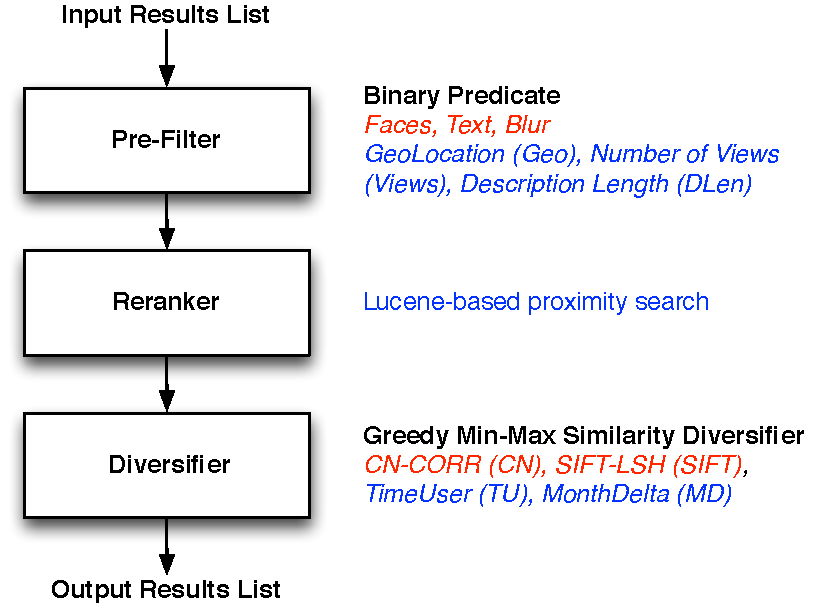
\includegraphics[width=0.9\columnwidth]{images/overview}
	\caption{\label{fig:overview}Overall workflow for diversify results}
\end{figure}

\subsection{Pre-Filters}
We removed many of the images which weren't relevant using some of our pre-filters before diversifying them. Images which contained frontal or side view of faces in focus were discarded and we also got rid of the blurred out-of-focus ones. Images were further checked for the amount of text they contained and those with high percentage were thrown away. Those images which had been geotagged more than 8~km away from their actual location were removed. We found that images without any views were usually not relevant and so only took into consideration those which had more than 2 views. Similarly we discovered that images with very large descriptions tend to be irrelevant and hence filtered out those whose descriptions were over 2000 characters long.

\begin{table*}[t!]
	\caption{\label{tab:conf}Run configuration}
	\centering
\begin{subtable}{0.9\columnwidth}
	\centering
\begin{tabular}{|l||c|c|c|c|c|c|}
	\hline
	& \multicolumn{3}{c|}{Visual} & \multicolumn{3}{c|}{Meta/Textual} \\
Run	& Face & Blur & Text & Geo & Views & DLen \\
	\hline
1 & \checkmark & \checkmark & \checkmark &   &   &   \\
	\hline
2 &   &   &   & \checkmark & \checkmark & \checkmark \\
	\hline
3 &   & \checkmark & \checkmark & \checkmark & \checkmark & \checkmark \\
	\hline
\end{tabular}
\caption{\label{tab:filters}Pre-filters applied in each of the runs.}
\end{subtable}
~
\begin{subtable}{0.9\columnwidth}
	\centering
\begin{tabular}{|l||c|c|c|c|c|}
	\hline
	& & \multicolumn{2}{c|}{Visual} & \multicolumn{2}{c|}{Meta/Textual} \\
Run	& Reranker & CN & SIFT & TU & MD \\
	\hline
1 &   & \checkmark &   &   &  \\
	\hline
2 & \checkmark &   &   & \checkmark & \checkmark \\
	\hline
3 & \checkmark &  & \checkmark & \checkmark & \checkmark \\
	\hline
\end{tabular}
\caption{\label{tab:feat}Reranker and features in each of the runs.}
\end{subtable}
\end{table*}

% \begin{table*}[ht]
% 	\caption{\label{tab:results}Official Results}
% 	\begin{subtable}{\textwidth}
% 	\centering
% 	\begin{tabular}{|l||c|c|c||c|c|c||c|c|c|}
% 		\hline
% 		 & \multicolumn{3}{c|}{ALL} & \multicolumn{3}{c||}{Keywords} & \multicolumn{3}{c|}{KeywordsGPS} \\
% 		Run & P@10 & CR@10 & F1@10 & P@10 & CR@10 & F1@10 & P@10 & CR@10 & F1@10 \\
% 		\hline\hline
% 		1 & 0.6994 & 0.4081 & 0.4926 & 0.6106 & 0.4075 & 0.462 & 0.7552 & 0.4085 & 0.5119 \\
% 		\hline
% 		2 & 0.8231 & 0.4306 & 0.5397 & 0.7667 & 0.4527 & 0.5379 & 0.8586 & 0.4166 & 0.5408 \\
% 		\hline
% 		3 & 0.8158 & 0.4398 & 0.5455 & 0.7561 & 0.4655 & 0.5461 & 0.8533 & 0.4236 & 0.5451 \\
% 		\hline
% 	\end{tabular}
% 	\caption{\label{tab:expertResults}Results using the expert groundtruth}
% 	\end{subtable}
% \\
% 	\begin{subtable}{\textwidth}
% 	\centering
% 	\begin{tabular}{|l||c||c|c||c|c||c|c|}
% 		\hline
% 		 &  & \multicolumn{2}{c||}{GT1} & \multicolumn{2}{c||}{GT2} & \multicolumn{2}{c|}{GT3} \\
% 		Run & P@10 & CR@10 & F1@10 & CR@10 & F1@10 & CR@10 & F1@10 \\
% 		\hline\hline
% 		1 & 0.6612 & 0.8174 & 0.7043 & 0.7858 & 0.688 & 0.6398 & 0.6197 \\
% 		\hline
% 		2 & 0.7694 & 0.8124 & 0.7689 & 0.7474 & 0.7276 & 0.6745 & 0.6944 \\
% 		\hline
% 		3 & 0.7714 & 0.8184 & 0.7734 & 0.7486 & 0.7263 & 0.668 & 0.6906 \\
% 		\hline
% 	\end{tabular}
% 	\caption{\label{tab:crowdResults}Results using groundtruth provided by three non-expert crowdworkers}
% 	\end{subtable}
% \end{table*}

\begin{table*}[ht]
	\centering
	\caption{\label{tab:results}Official Results}
	\begin{tabular}{|l|||c|c|c|||c||c|c||c|c||c|c|}
		\hline
		 & \multicolumn{3}{c|||}{Expert} &  \multicolumn{7}{c|}{Crowdworker}\\
		\hline
		 & \multicolumn{3}{c|||}{ALL} &  & \multicolumn{2}{c||}{GT1} & \multicolumn{2}{c||}{GT2} & \multicolumn{2}{c|}{GT3}\\
		Run & P@10 & CR@10 & F1@10 & P@10 & CR@10 & F1@10 & CR@10 & F1@10 & CR@10 & F1@10 \\
		\hline\hline
		1 & 0.6994 & 0.4081 & 0.4926 & 0.6612 & 0.8174 & 0.7043 & 0.7858 & 0.688 & 0.6398 & 0.6197 \\
		\hline
		2 & 0.8231 & 0.4306 & 0.5397 & 0.7694 & 0.8124 & 0.7689 & 0.7474 & 0.7276 & 0.6745 & 0.6944 \\
		\hline
		3 & 0.8158 & 0.4398 & 0.5455 & 0.7714 & 0.8184 & 0.7734 & 0.7486 & 0.7263 & 0.668 & 0.6906 \\
		\hline
	\end{tabular}
\end{table*}



\subsection{Reranker}
The original results lists provided in the task were retrieved by searching Flickr with a given monument name. The exact search implementation used by Flickr is unknown, but it is likely to be a variant of the vector space model with stemming. A better, more precise, ranking of the results can be achieved by performing a phrase or proximity search in which the results are scored higher if the query terms occur in close proximity in the metadata. To apply proximity-based reranking, we indexed the title, description and tags fields of each image in the filtered results list with Lucene, and performed the following query:
\begin{alltt}
\texttt{(TITLE:``\emph{monument}''~20 OR TAGS:``\emph{monument}''~20 OR 
  DESCRIPTION:``\emph{monument}''~20) OR
  (TITLE:``\emph{monument}'')^0.5 (TAGS:``\emph{monument}'')^0.1}
\end{alltt}

\subsection{Similarity Matrices}
In order to use the Min-Max diversifier, a similarity matrix is required. At the beginning of the task we spent some time analysing the data, and looking at features which could be sensibly used  to compute similarity. One particular problem we noticed was that many of the images had the same description and tags, even though they were visually diverse. %This is a result of the way many images are tagged and annotated on Flickr using so-called \emph{bulk tagging}. 
This means that standard techniques for diversification based on the text are unlikely to work well in many cases, and would in all likelihood end up to being similar to just diversifying based on the users that took the photo. With this in mind, we started to explore other features that could work better. 

\noindent \textbf{Color Naming Histogram} (CN). The provided CN histogram features~\cite{DIV2013}, were used to create a similarity matrix by using correlation to measure the pairwise similarity.

\noindent \textbf{Scale-Invariant Feature Transform} (SIFT). SIFT features from the images were extracted and hashed using an LSH scheme~\cite{Hare:2013:TVP:2461466.2461514}. A sparse binary similarity matrix was created from these, by setting a similarity of 1 to pairs of images in which there was a hash collision.

\noindent \textbf{Time User} (TU). Images taken by the same user within a short time period are likely to be similar. A similarity matrix was constructed with the following constraints: pairs of images taken a less than a minute apart had similarity 1; images more than 3.25 mins apart had 0 similarity. Between 1 and 3.25 minutes the similarity falls off logarithmically.

\noindent \textbf{Month Delta} (MD). Similar to the TU feature, images have increasing similarity with closer month of year.

\section{Experiments and Results}\label{sec:exp}
Three runs were submitted; their configuration with respect to the methodology and features described in Section~\ref{sec:meth} is illustrated in Tables~\ref{tab:filters} and~\ref{tab:feat}. Where multiple features were used, the similarity matrices were just averaged to create a single matrix. Two major points can be noted from the results. Firstly, using textual and visual features outperforms the use of either modality alone with our techniques. It is also clear that the reranking stage massively helps improve precision. Secondly, the high variability in results across the experts and crowdworkers indicates that the task is actually rather subjective; it is particularly interesting that when compared against the crowdworker groundtruths our cluster recall scores are almost double, perhaps indicating that the experts tended to over-segment the result sets.

\section{Acknowledgments}
The described work was funded by the European Union Seventh Framework Programme (FP7/2007-2013) under grant agreements 270239 (ARCOMEM), and 287863 (TrendMiner).


\bibliographystyle{abbrv}
\bibliography{../bibliography}
\end{document}
